\documentclass{article}%
\usepackage[T1]{fontenc}%
\usepackage[utf8]{inputenc}%
\usepackage{lmodern}%
\usepackage{textcomp}%
\usepackage{lastpage}%
\usepackage[head=40pt,margin=0.5in,bottom=0.6in]{geometry}%
\usepackage{graphicx}%
%
\title{\textbf{Trabajadores del sector público protestaron en la Plaza Morelos}}%
\author{El Nacional Web}%
\date{28/11/2018}%
%
\begin{document}%
\normalsize%
\maketitle%
\textbf{URL: }%
http://www.el{-}nacional.com/noticias/protestas/trabajadores{-}del{-}sector{-}publico{-}protestaron{-}plaza{-}morelos\_261377\newline%
%
\textbf{Periodico: }%
EN, %
ID: %
261377, %
Seccion: %
Protestas\newline%
%
\textbf{Palabras Claves: }%
NO\_TIENE\newline%
%
\textbf{Derecho: }%
2.3, %
Otros Derechos: %
, %
Sub Derechos: %
2.3.4\newline%
%
\textbf{EP: }%
SI\newline%
\newline%
%
\textbf{\textit{Empleados del Instituto Nacional del Deporte, Cantv, Metro de Caracas, Movilnet y otras empresas acudieron a la manifestación~}}%
\newline%
\newline%
%
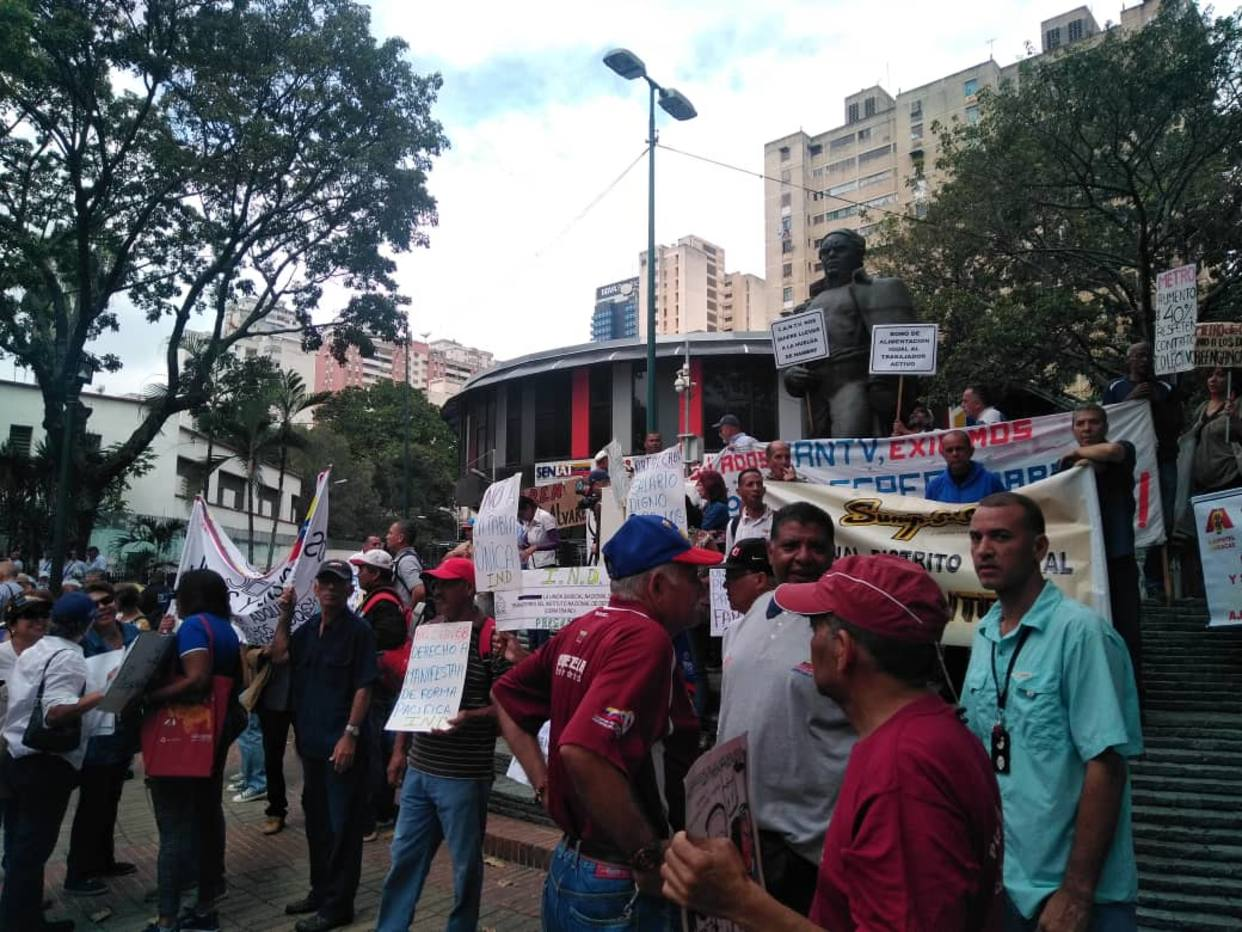
\includegraphics[width=300px]{194.jpg}%
\newline%
%
Trabajadores del sector público protestaron este miércoles en la Plaza Morelos de Caracas para consignar un documento en la Defensoría del Pueblo y exigir mejoras salariales y laborales.%
\newline%
%
En la manifestación se concentraron empleados del Instituto Nacional del Deporte, Metro Caracas; Corpoelec, Cantv, Movilnet, Petroleros, Seniat y otras empresas estatales.%
\newline%
%
Además, los empleados de diversos sectores de trabajo exigieron pagos a jubilados, el cumplimiento de los contratos colectivos y las reivindicaciones salariales por los años de servicio en las distintas empresas.%
\newline%
%
Un piquete de la Guardia Nacional Bolivariana impidió el trayecto de los trabajadores a la Defensoría del Pueblo.%
\newline%
%
\end{document}